\documentclass{article}
%\usepackage[english]{babel}%
\usepackage{graphicx}
\usepackage{tabulary}
\usepackage{tabularx}
\usepackage[normalem]{ulem}
\usepackage{cancel}
\usepackage{tikz} 
\usepackage{pdflscape}
\usepackage{colortbl}
\usepackage{lastpage}
\usepackage{multirow}
\usepackage{enumerate}
\usepackage{color,soul}
\usepackage{pdflscape}
\usepackage{hyperref}
%\usepackage[table]{xcolor}
\usepackage{rotating}
\usepackage{amsmath}
\usepackage{fixltx2e}
\usepackage{framed}
\usepackage{mdframed}
\usepackage[T1]{fontenc}
\usepackage[utf8]{inputenc}
\usepackage{textcomp}
\usepackage{siunitx}
\usepackage{ifthen}
\usepackage{fancyhdr}
\usepackage{gensymb}
 \usepackage{newunicodechar}
\usepackage[document]{ragged2e}
\usepackage[margin=1in,top=1.2in,headheight=57pt,headsep=0.1in]
{geometry}
\usepackage{ifthen}
\usepackage{fancyhdr}
\everymath{\displaystyle}
\usepackage[document]{ragged2e}
\usepackage{fancyhdr}
\everymath{\displaystyle}
%\usepackage[table,xcdraw]{xcolor}
\usetikzlibrary{calc}
\usetikzlibrary{arrows}
\linespread{2}%controls the spacing between lines. Bigger fractions means crowded lines%
%\pagestyle{fancy}
%\usepackage[margin=1 in, top=1in, includefoot]{geometry}
%\everymath{\displaystyle}
\linespread{1.3}%controls the spacing between lines. Bigger fractions means crowded lines%
%\pagestyle{fancy}
\pagestyle{fancy}
\setlength{\headheight}{56.2pt}


\chead{\ifthenelse{\value{page}=1}{
\includegraphics[scale=0.3]{SCC}\\ \textbf \textbf WATR048 - Practice Math Set 1 of 2}}
\rhead{\ifthenelse{\value{page}=1}{Shabbir Basrai}{Shabbir Basrai}}
\lhead{\ifthenelse{\value{page}=1}{WATR 048 - Fall 2021}{\textbf WATR048 - Practice Math Set 1 of 2}}
\rfoot{\ifthenelse{\value{page}=1}{}{WATR 048 - Fall 2021}}

\cfoot{}
\lfoot{Page \thepage\ of \pageref{LastPage}}
\renewcommand{\headrulewidth}{2pt}
\renewcommand{\footrulewidth}{1pt}
\begin{document}
%_______________________________________________________________________________________________________________________________________%


\section{Unit Conversions}\index{Unit Conversions}
\subsection{Example Problems} \index{Example Problems}  
\begin{enumerate}
\item Convert 1000 $ft^3$ to cu. yards:\\
$1000 \cancel{ft^3}*\dfrac{cu.yards}{27\cancel{ft^3}} = 37 cu.yards$\\

\item Convert 3.5 $ft^3/sec$ to MGD:\\
$\dfrac{3.5 \enspace \cancel{ft^3}}{\cancel{sec}} * \dfrac{7.48\cancel {\enspace gal}}{\cancel{ft^3}} * \dfrac{MG}{\enspace 10^6 \cancel{gal}}* \dfrac{1440*60 \enspace \cancel{sec}}{day}=  2.3 \enspace MGD$\\

\item Convert 1,000 L water to lbs:\\
$1000 \enspace \cancel{L}*\dfrac {\cancel{gal}}{3.785 \enspace \cancel{L}}*\dfrac{8.34 \enspace lbs}{\cancel{gal}}\enspace  = 2,203 \enspace lbs$\\
$(Note:8.34 \enspace lbs/gal \enspace is \enspace density \enspace of \enspace water - a \enspace constant)$\\ 
\end{enumerate}


\subsection{Practice Problems} \index{Practice Problems}
\begin{enumerate}
\item Given 1 ft = 30.48 cm and 5,280 ft = mile, convert 3 miles to cm\\
Solution:\\
$3 \enspace \cancel{miles} * \dfrac{5,280 \enspace \cancel{ft}}{\cancel{mile}}*\dfrac{30.48 \enspace cm}{\cancel{ft}}=\boxed{482,803 \enspace cm}$

\item The wastewater flow to a treatment plant has a velocity of 61 cm/s. What is this velocity expressed in ft/min. Given: 1 ft = 30.48 cm\\
Solution:\\
$61 \enspace \dfrac{\cancel{cm}}{\cancel{s}} * \dfrac{ft}{30.48 \enspace \cancel{cm}}* \dfrac{60 \enspace \cancel{s}}{min} =  \boxed{120 \enspace ft/min}$\\

\item As an operator of a wastewater plant you are treating a flow of 21 MGD, what is the flow in gallons per minute?\\
Solution:\\
$\dfrac{21 \cancel{MG}}{\cancel{day}}*\dfrac{1,000,000 \enspace gal}{\cancel{MG}}*\dfrac{\cancel{day}}{24*60 \enspace min}=\boxed{\dfrac{14,583 \enspace gal}{min}}$\\
\end{enumerate}

\newpage

\section{Area \& Volume}\index{Area \& Volume}
% \section{Area \& Volume}\index{Area \& Volume}

% \begin{snugshade*}
% 	\item \noindent\textsc{Area \& Volume}
% \end{snugshade*}
 
\subsection{Example Problems} \index{Example Problems} 
% \hl{Example Problems}\\
\begin{enumerate}


\item The floor of a rectangular building is 20 feet long by 12 feet wide and the inside walls are 10 feet high. Find the total surface area of the inside walls of this building\\
Solution:\\
\begin{center}
\begin{tikzpicture}
	%%% Edit the following coordinate to change the shape of your
	%%% cuboid
      
	%% Vanishing points for perspective handling
	\coordinate (P1) at (-7cm,1.5cm); % left vanishing point (To pick)
	\coordinate (P2) at (8cm,1.5cm); % right vanishing point (To pick)

	%% (A1) and (A2) defines the 2 central points of the cuboid
	\coordinate (A1) at (0em,0cm); % central top point (To pick)
	\coordinate (A2) at (0em,-2cm); % central bottom point (To pick)

	%% (A3) to (A8) are computed given a unique parameter (or 2) .8
	% You can vary .8 from 0 to 1 to change perspective on left side
	\coordinate (A3) at ($(P1)!.8!(A2)$); % To pick for perspective 
	\coordinate (A4) at ($(P1)!.8!(A1)$);

	% You can vary .8 from 0 to 1 to change perspective on right side
	\coordinate (A7) at ($(P2)!.7!(A2)$);
	\coordinate (A8) at ($(P2)!.7!(A1)$);

	%% Automatically compute the last 2 points with intersections
	\coordinate (A5) at
	  (intersection cs: first line={(A8) -- (P1)},
			    second line={(A4) -- (P2)});
	\coordinate (A6) at
	  (intersection cs: first line={(A7) -- (P1)}, 
			    second line={(A3) -- (P2)});

	%%% Depending of what you want to display, you can comment/edit
	%%% the following lines

	%% Possibly draw back faces

	\fill[gray!40] (A2) -- (A3) -- (A6) -- (A7) -- cycle; % face 6
	\node at (barycentric cs:A2=1,A3=1,A6=1,A7=1) {\tiny Floor=W*L};
	
	\fill[gray!50] (A3) -- (A4) -- (A5) -- (A6) -- cycle; % face 3
	\node at (barycentric cs:A3=1,A4=1,A5=1,A6=1) {\tiny Wall - W*H};
	
	\fill[gray!10, opacity=0.2] (A5) -- (A6) -- (A7) -- (A8) -- cycle; % face 4
	\node at (barycentric cs:A5=1,A6=1,A7=1,A8=1) {\tiny Wall - L*H};
	
	\fill[gray!10,opacity=0.5] (A1) -- (A2) -- (A3) -- (A4) -- cycle; % f2
	\node at (barycentric cs:A1=1,A2=1,A3=1,A4=1) {\tiny Wall - L*H};
	
	\fill[gray!40,opacity=0.2] (A1) -- (A4) -- (A5) -- (A8) -- cycle; % f5
	\node at (barycentric cs:A1=1,A4=1,A5=1,A8=1) {\tiny Ceiling=W*L};	
	
	\draw[thick,dashed] (A5) -- (A6);
	\draw[thick,dashed] (A3) -- (A6);
	\draw[thick,dashed] (A7) -- (A6);

	%% Possibly draw front faces

	%\fill[orange] (A1) -- (A8) -- (A7) -- (A2) -- cycle; % face 1
	\node at (barycentric cs:A1=1,A8=1,A7=1,A2=1) {\tiny Wall - W*H};
	


	%% Possibly draw front lines
	\draw[thick] (A1) -- (A2);

	\draw[<->] (-1.8,0.38) -- (-1.8,-1.3)node [midway, above=-1.8mm] {\hspace{-1.3cm}\tiny Height=10'};
	\draw[<->] (-1.6,-1.4) -- (-.3,-2.1)node [midway, above=-2.6mm] {\hspace{-1.3cm}\tiny Length=20'};
	\draw[<->] (2.6,-1.13) -- (0.2,-2.2)node [midway, below=.6mm] {\hspace{1.2cm}\tiny Width=12'};
	\draw[thick] (A3) -- (A4);
	\draw[thick] (A7) -- (A8);
	\draw[thick] (A1) -- (A4);
	\draw[thick] (A1) -- (A8);
	\draw[thick] (A2) -- (A3);
	\draw[thick] (A2) -- (A7);
	\draw[thick] (A4) -- (A5);
	\draw[thick] (A8) -- (A5);
	
	% Possibly draw points
	% (it can help you understand the cuboid structure)
%	\foreach \i in {1,2,...,8}
%	{
%	  \draw[fill=black] (A\i) circle (0.15em)
%	    node[above right] {\tiny \i};
%	}
	% \draw[fill=black] (P1) circle (0.1em) node[below] {\tiny p1};
	% \draw[fill=black] (P2) circle (0.1em) node[below] {\tiny p2};
\end{tikzpicture}\\
\end{center}
2 Walls W*H + 2 Walls L*H= $2*12*10ft^2 + 2*20*10ft^2$\\
$=240+400=\boxed{640ft^2}$\\

2 Walls W*H + 2 Walls L*H + Floor + Ceiling= $2*12*10ft^2 + 2*20*10ft^2 + 2*12*20ft^2$\\
$=240+400+480=\boxed{1,120ft^2}$\\




\item What is the surface area of a cylinder 50 ft diameter and 25 ft height?\\
Solution:\\
\begin{center}
\begin{tikzpicture}[mydashed/.style={dashed,dash phase=2pt}]
\draw (0,0) ellipse (2cm and 0.3cm) node [midway, above=-2.4mm] {\hspace{0.1cm}\tiny{Top Area$=\dfrac{\pi}{4}*D^2$}};
\draw (0,-2.3) ellipse (2cm and 0.3cm) node [midway, below=2.05cm] {\hspace{0.1cm}\tiny{Bottom Area$=\dfrac{\pi}{4}*D^2$}};
\draw [-] (2,-2.3) -- (2,0);
%\draw [<->] (-2,0) -- (2,0); 
\draw [<->] (2.5,-2.3) -- (2.5,0) node [midway, below] {\hspace{2.9cm}Height (h) =25'};
\draw [<->] (-2,-0.4) -- (2,-0.4) node [midway, below=0.7mm] {\hspace{0.1cm}\small{Diameter (D)=50'}};
%\draw [-] (0,-4) -- (2,-2.3);
%\draw [-] (0,-4) -- (-2,-2.3);
%\draw [-] (0,-4) -- (2,-2.3);
\draw [-] (-2,0) -- (-2,-2.3) node [midway, below] {\hspace{4cm}\tiny{Cylinder Surface Area$=\pi*D*h$}};
\draw [-latex, mydashed, line width=1mm, rotate=-90] (0.6,-1.9) arc [start angle=-120, end angle=120, x radius=0.8cm, y radius=2.2cm];
%\draw [-latex, thick, rotate=-95] (0,0) arc [start angle=-190, end angle=160, x radius=1cm, y radius=2cm];
\end{tikzpicture}\\
\end{center}
$Surface \enspace area \enspace of \enspace cylinder=surface \enspace area \enspace of \enspace the \enspace top \enspace  and \enspace bottom \enspace faces + surface \enspace area \enspace of \enspace the \enspace cylinder$\\
$\implies(2*\dfrac{\pi}{4}*D^2)+(\pi*D*h)=2*0.785*50^2+3.14*50*25=\boxed{7,850ft^2}$
\end{enumerate}






\subsection{Practice Problems} \index{Practice Problems}
\begin{enumerate}

\item A cylindrical tank is 10 feet in diameter and 20 feet in height. 'What is the approximate capacity in liters?\\
Solution:\\

\begin{tikzpicture}
\draw (0,0) ellipse (2cm and 0.3cm);
\draw (0,-2.3) ellipse (2cm and 0.3cm);
\draw [-] (2,-2.3) -- (2,0);
\draw [<->] (-2,0) -- (2,0) node [midway, above=3mm] {\hspace{0.1cm}Diameter=10'}; 
\draw [<->] (2.5,-2.3) -- (2.5,0) node [midway, below] {\hspace{1.9cm}Height=20'};
%\draw [-] (0,-4) -- (2,-2.3);
%\draw [-] (0,-4) -- (-2,-2.3);
%\draw [-] (0,-4) -- (2,-2.3);
\draw [-] (-2,0) -- (-2,-2.3);
\end{tikzpicture}\\

$Volume=\dfrac{\pi}{4}D^2*H=0.785*10^2*20\cancel{ft^3}*7.48\dfrac{\cancel{gallons}}{\cancel{ft^3}}*3.78\dfrac{liters}{\cancel{gallons}}=\boxed{44,462 \enspace liters}$

\item What is the volume of water in a sedimentation basin 80 feet long, 28 feet wide and a 9.5 feet water depth? Give your answer in gallons.\\
Solution:\\
$Volume=80*28*9.5 \cancel{ft^3}*7.48\dfrac{gallons}{\cancel{ft^3}}=\boxed{159,174 \enspace gallons} $

\item How many gallons will 1,200 feet of 6-inch pipe hold?\\
Solution:\\
\begin{center}
\begin{tikzpicture}
\draw (0,0) ellipse (0.1cm and 0.3cm);
\draw (10,0) ellipse (0.1cm and 0.3cm);
\draw [-] (0,-0.29) -- (10,-0.29);
\draw [-] (0,0.29) -- (10,0.29);
\draw [<->] (10,-0.28) -- (10,0.28) node [midway, below=-3mm] {\hspace{2.6cm}Diameter=6"};
\draw [<->] (0,-.68) -- (10,-.68)node [midway, below] {\hspace{0.9cm}Length=1,200'};
\end{tikzpicture}
\end{center}
$Volume=\dfrac{\pi}{4}D^2*L=0.785*\Big(\dfrac{6}{12}\Big)^2*1200\cancel{ft^3}*7.48\dfrac{gallons}{\cancel{ft^3}}=\boxed{1,762 \enspace gallons}$

\item What is the surface area of a cylinder 80 ft diameter and 25 ft height?  Cylindrical part surface area only. Disregard the floor and roof areas.\\
Solution:\\
\begin{center}
\begin{tikzpicture}[mydashed/.style={dashed,dash phase=2pt}]
\draw (0,0) ellipse (2cm and 0.3cm) node [midway, above=-2.4mm] {};
\draw (0,-2.3) ellipse (2cm and 0.3cm) node [midway, below=2.05cm] {};
\draw [-] (2,-2.3) -- (2,0);
%\draw [<->] (-2,0) -- (2,0); 
\draw [<->] (2.5,-2.3) -- (2.5,0) node [midway, below] {\hspace{2.9cm}Height (h) = 25'};
\draw [<->] (-2,-0.4) -- (2,-0.4) node [midway, below=0.7mm] {\hspace{0.1cm}\small{Diameter (D)}=80'};
%\draw [-] (0,-4) -- (2,-2.3);
%\draw [-] (0,-4) -- (-2,-2.3);
%\draw [-] (0,-4) -- (2,-2.3);
\draw [-] (-2,0) -- (-2,-2.3) node [midway, below] {\hspace{4cm}\tiny{Cylinder Surface Area$=\pi*D*h$}};
\draw [-latex, mydashed, line width=1mm, rotate=-90] (0.6,-1.9) arc [start angle=-120, end angle=120, x radius=0.8cm, y radius=2.2cm];
%\draw [-latex, thick, rotate=-95] (0,0) arc [start angle=-190, end angle=160, x radius=1cm, y radius=2cm];
\end{tikzpicture}\\
\end{center}
$Surface \enspace area \enspace of \enspace cylinder=\pi*D*h=3.14*80*25=\boxed{6,280ft^2}$

\item If the surface area of a clarifier is 5,025$ft^2$, what is its circumference?\\
Solution:\\
$Surface \enspace area=\dfrac{\pi}{4}*D^2 \enspace \implies 5025ft^2=0.785*D^2 ft^2\implies D^2=\dfrac{5025}{0.785} \implies D=\sqrt{6401.3}=80ft \implies \enspace Circumference=\pi*D=3.14*80ft=\boxed{251ft}$

\item How many gallons of paint will be required to paint the inside walls of a 40 ft long x 65 ft wide x 20 ft high tank if the paint coverage is 150 sq. ft per gallon.  Note:  We are painting walls only.  Disregard the floor and roof areas.\\
Solution:\\
\begin{center}
\begin{tikzpicture}
	%%% Edit the following coordinate to change the shape of your
	%%% cuboid
      
	%% Vanishing points for perspective handling
	\coordinate (P1) at (-7cm,1.5cm); % left vanishing point (To pick)
	\coordinate (P2) at (8cm,1.5cm); % right vanishing point (To pick)

	%% (A1) and (A2) defines the 2 central points of the cuboid
	\coordinate (A1) at (0em,0cm); % central top point (To pick)
	\coordinate (A2) at (0em,-2cm); % central bottom point (To pick)

	%% (A3) to (A8) are computed given a unique parameter (or 2) .8
	% You can vary .8 from 0 to 1 to change perspective on left side
	\coordinate (A3) at ($(P1)!.8!(A2)$); % To pick for perspective 
	\coordinate (A4) at ($(P1)!.8!(A1)$);

	% You can vary .8 from 0 to 1 to change perspective on right side
	\coordinate (A7) at ($(P2)!.7!(A2)$);
	\coordinate (A8) at ($(P2)!.7!(A1)$);

	%% Automatically compute the last 2 points with intersections
	\coordinate (A5) at
	  (intersection cs: first line={(A8) -- (P1)},
			    second line={(A4) -- (P2)});
	\coordinate (A6) at
	  (intersection cs: first line={(A7) -- (P1)}, 
			    second line={(A3) -- (P2)});

	%%% Depending of what you want to display, you can comment/edit
	%%% the following lines

	%% Possibly draw back faces

	\fill[gray!40] (A2) -- (A3) -- (A6) -- (A7) -- cycle; % face 6
	\node at (barycentric cs:A2=1,A3=1,A6=1,A7=1) {};
	
	\fill[gray!50] (A3) -- (A4) -- (A5) -- (A6) -- cycle; % face 3
	\node at (barycentric cs:A3=1,A4=1,A5=1,A6=1) {\tiny Wall - W*H};
	
	\fill[gray!10, opacity=0.2] (A5) -- (A6) -- (A7) -- (A8) -- cycle; % face 4
	\node at (barycentric cs:A5=1,A6=1,A7=1,A8=1) {\tiny Wall - L*H};
	
	\fill[gray!10,opacity=0.5] (A1) -- (A2) -- (A3) -- (A4) -- cycle; % f2
	\node at (barycentric cs:A1=1,A2=1,A3=1,A4=1) {\tiny Wall - L*H};
	
	\fill[gray!40,opacity=0.2] (A1) -- (A4) -- (A5) -- (A8) -- cycle; % f5
	\node at (barycentric cs:A1=1,A4=1,A5=1,A8=1) {};	
	
	\draw[thick,dashed] (A5) -- (A6);
	\draw[thick,dashed] (A3) -- (A6);
	\draw[thick,dashed] (A7) -- (A6);

	%% Possibly draw front faces

	%\fill[orange] (A1) -- (A8) -- (A7) -- (A2) -- cycle; % face 1
	\node at (barycentric cs:A1=1,A8=1,A7=1,A2=1) {\tiny Wall - W*H};
	


	%% Possibly draw front lines
	\draw[thick] (A1) -- (A2);

	\draw[<->] (-1.8,0.38) -- (-1.8,-1.3)node [midway, above=-1.8mm] {\hspace{-1.3cm}\tiny Height=20'};
	\draw[<->] (-1.6,-1.4) -- (-.3,-2.1)node [midway, above=-2.6mm] {\hspace{-1.3cm}\tiny Length=45'};
	\draw[<->] (2.6,-1.13) -- (0.2,-2.2)node [midway, below=.6mm] {\hspace{1.2cm}\tiny Width=65'};
	\draw[thick] (A3) -- (A4);
	\draw[thick] (A7) -- (A8);
	\draw[thick] (A1) -- (A4);
	\draw[thick] (A1) -- (A8);
	\draw[thick] (A2) -- (A3);
	\draw[thick] (A2) -- (A7);
	\draw[thick] (A4) -- (A5);
	\draw[thick] (A8) -- (A5);
	
	% Possibly draw points
	% (it can help you understand the cuboid structure)
%	\foreach \i in {1,2,...,8}
%	{
%	  \draw[fill=black] (A\i) circle (0.15em)
%	    node[above right] {\tiny \i};
%	}
	% \draw[fill=black] (P1) circle (0.1em) node[below] {\tiny p1};
	% \draw[fill=black] (P2) circle (0.1em) node[below] {\tiny p2};
\end{tikzpicture}\\
\end{center}
2 Walls W*H + 2 Walls L*H = $2*65*20ft^2 + 2*40*20ft^2= 2,600+1,600=4,200ft^2$\\
$\implies @150\dfrac{ft^2}{gal} \enspace paint \enspace coverage \enspace \rightarrow \enspace \dfrac{4,200\cancel{ft^2}}{150\dfrac{\cancel{ft^2}}{gal}}=\boxed{28 \enspace gallons}$

\item What is the circumference of a 100 ft diameter circular clarifier?\\
Solution:\\
$Circumference=\pi*D=3.14*100ft=\boxed{314ft}$

\item If the surface area of a clarifier is 5,025$ft^2$, what is its diameter?\\
Solution:\\
$Surface \enspace area=\dfrac{\pi}{4}*D^2 \enspace \implies 5025ft^2=0.785*D^2 ft^2\implies D^2=\dfrac{5025}{0.785} \implies D=\sqrt{6401.3}=\boxed{80ft}$

\end{enumerate}

\section{Concentration}\index{Concentration}
% \section{Area \& Volume}\index{Area \& Volume}

% \begin{snugshade*}
% 	\item \noindent\textsc{Area \& Volume}
% \end{snugshade*}
 
\subsection{Example Problems} \index{Example Problems}
\begin{enumerate}
\item What is the salt content in mg/l of a 2.5\% salt solution?\\
Solution:
25,000mg/l
\item What is the \% concentration of a solids content in a sludge with 5000 mg/l solids concentration?\\
Solution:\\
0.5\%\\
\end{enumerate}
\subsection{Practice Problems} \index{Practice Problems}

\begin{enumerate}
\item A 6.35\% solution is is equivalent to {\underline{\hspace{1cm}}} mg/l\\
Answer:\\
63,500 mg/l\\
\end{enumerate}
\vspace{0.3cm}


























\section{Flow and Velocity}\index{Flow and Velocity}
\begin{enumerate}
\item Calculate the velocity of a 14 MGD flow in a 6 ft wide channel with a water depth of two feet.\\
\begin{center}
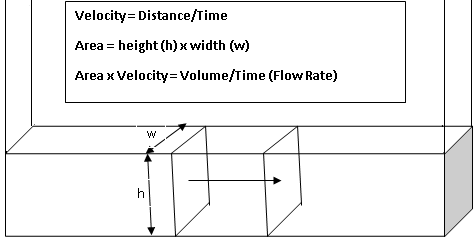
\includegraphics[scale=0.5]{ChannelFlow3}
\end{center}
$Flow (Q) = Velocity (V) * Area (A)$\\
$\implies Flow\Big[ 14 \dfrac{MG}{day}* \dfrac{10^6 gal}{MG} * \dfrac{ft^3}{7.48 gal}*\dfrac{day}{24*60*60sec}\Big]\dfrac{ft^3}{sec} = Velocity(V) \dfrac{ft}{sec}* Area (6 * 2) ft ^2$\\
\vspace{0.2cm}
$\implies 21.7 \dfrac{ft^3}{sec}= V\dfrac{ft}{sec}*12ft^2$\\
$\implies V \dfrac{ft}{sec}= \dfrac{21.7\dfrac{\cancelto{ft}{ft^3}}{sec}}{12\cancelto{}{ft^2}}= \boxed{1.8\dfrac{ft}{sec}}$\\

\item If a chemical is added in a sewer where wastewater is flowing at a velocity of 3.1 feet per second, how many minutes would it take for the chemical to reach the plant 7 miles away?\\
Solution:\\
Min $= \dfrac{1}{3.1}\dfrac{sec}{ft}*\dfrac{5280ft}{mile}*7 miles*\dfrac{min}{60 sec} = \boxed{199 min}$
\\

\item A plastic float takes 9.8 seconds to travel a distance of 25 feet in a wastewater channel. The channel is 3 ft 8 in. wide and the water level in this channel is 28 inches. What is the wastewater flow in GPM\\
Solution:\\
\vspace{0.3cm}
$Q=V*A$\\
$\implies Q=\dfrac{25ft}{9.8s}*\Big((3+\dfrac{8}{12})*\dfrac{28}{12}\Big)ft^2*7.48\dfrac{gal}{ft^3}*60\dfrac{s}{min}=\boxed{9,795\dfrac{gal}{min}}$



\item Calculate the flow, in gpd, that would pass through a grit chamber 2 feet wide, at a depth of 6 inches, with a velocity of 1 ft /sec\\
a. 646,272gpd \\
b. 610,000gpd \\
c. 300,272gpd \\
d. 576,534gpd \\
Solution:\\
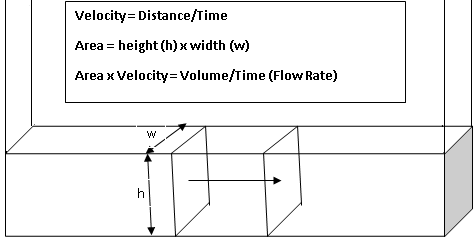
\includegraphics[scale=0.5]{ChannelFlow3}\\
$Q=V*A$\\
$Q=1\dfrac{ft}{s}*(2*0.5)ft^2=1\dfrac{ft^3}{s}$\\
$Q=1\dfrac{\cancel{ft^3}}{\cancel{s}}*\dfrac{(1440*60)\cancel{s}}{day}*7.48\dfrac{gal}{\cancel{ft^3}}=\boxed{646,272\dfrac{gal}{day}}$
\end{enumerate}



\subsection{Practice Problems} \index{Practice Problems}

\begin{enumerate}
\item A wastewater channel is 3.25 feet wide and is conveying a wastewater flow of 3.5 MGD. The wastewater flow is 8 inches deep. Calculate the velocity of this flow.\\
Solution:\\
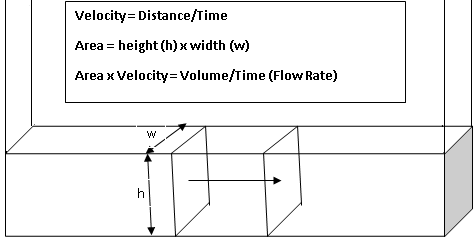
\includegraphics[scale=0.5]{ChannelFlow3}\\
$Q=V*A \implies V=\dfrac{Q}{A}$\\
$\implies V\dfrac{ft}{s}=\dfrac{3.5\dfrac{\cancel{MG}}{\cancel{day}}*\dfrac{1000000\cancel{gal}}{\cancel{MG}}*\dfrac{ft^{\cancel{3}}}{7.48\cancel{gal}}*\dfrac{\cancel{day}}{(1440*60)s}}{(3.25*0.75)\cancel{ft^2}}=\boxed{2.2\dfrac{ft}{s}}$

\item A plastic float is dropped into a wastewater channel and is found to travel 10 feet in 4.2 seconds. The channel is 2.4 feet wide and is flowing 1.8 feet deep. Calculate the flow rate of this wastewater in cubic feet per second.\\
Solution:\\
$Q=V*A$\\
$\implies Q\Big(\dfrac{ft^3}{s}\Big)=\dfrac{10ft}{4.2s}*(2.4*1.8)ft^2=\boxed{10.3\dfrac{ft^3}{s}}$
\item A 12 inch pipe conveys sewage at 2.6 feet per second.  What is the flow expressed in MGD?
Solution:\\
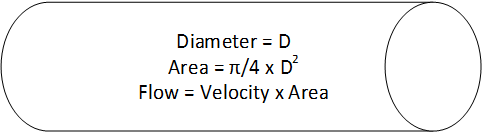
\includegraphics[scale=0.5]{PipeFlow}\\
$Q=V*A$\\
$Q=2.6\dfrac{\cancel{ft}}{\cancel{s}}*0.785*1^2\cancel{ft^2}*7.48\dfrac{\cancel{gal}}{ft^3}*\dfrac{MG}{1,000,000\cancel{gal}}*\dfrac{(1440*60)\cancel{s}}{day}=\boxed{1.3MGD}$\\

\item A sewer line to a wastewater treatment plant is 12 miles long. If the wastewater is flowing at 2.2 fps, approximately.  How long will it take for wastewater to reach the plant?\\
Solution:\\
$time \enspace to \enspace reach \enspace plant \enspace (hrs)=\dfrac{\cancel{s}}{2.2\cancel{ft}}*\dfrac{5280\cancel{ft}}{\cancel{mile}}*12\cancel{miles}*\dfrac{hrs}{(60*60)\cancel{s}}=\boxed{8hrs}$  
\end{enumerate}






















\section{Primary Treatment} \index{Primary Treatment}
\subsection{Example Problems} \index{Example Problems}
\begin{enumerate}
\item If a clarifier has a capacity of 0.25 MG, what is the detention time in hours if it receives a flow of 3 MGD\\
Solution:\\
$Clarifier \enspace detention \enspace time \enspace (hr) = 	\dfrac{ Clarifier \enspace volume (MG)}{Influent \enspace flow \enspace (MG/hr)}$\\
\vspace{0.5cm}
$Clarifier \enspace detention \enspace time \enspace (hr) = 	\dfrac{0.25\cancel{MG}}{\dfrac{3\cancel{MG}}{\cancel{day}}*\dfrac{\cancel{day}}{24hrs}}=\boxed{2hrs}$\\

\item If a 90 ft diameter primary clarifier operating at water depth of 20 ft is treating a 12MGD flow, calculate the surface loading rate (gal/(day-sq.ft).\\
Solution:\\
$Clarifier \enspace hydraulic \enspace loading \enspace 	\Big(\dfrac{gpd}{ft^2}\Big) =\dfrac{\dfrac{12\cancel{MG}}{{day}}*\dfrac{10^6gal}{\cancel{MG}}}{0.785*90^2 ft^2}=\boxed{1,887gpd/ft^2}$\\


\vspace{0.5cm}
\item What is the weir overflow rate (gpd/ft) when treating a 15 MGD flow in a 105 ft diameter primary sedimentation tank operating at water depth of 20 ft.\\
\vspace{0.5cm}
Solution:\\
\vspace{0.5cm}
$Clarifier \enspace detention \enspace time \enspace (hr) = 	\dfrac{(0.785*105^2*20)\cancel{ft^3}}{\dfrac{15\cancel{MG}}{\cancel{day}}*\dfrac{10^6\cancel{gal}}{\cancel{MG}}*\dfrac{\cancel{ft^3}}{7.48\cancel{gal}}*\dfrac{\cancel{day}}{24hrs}}=\boxed{2.1hrs}$\\
\end{enumerate}

\subsection{Practice Problems} \index{Practice Problems}

\begin{enumerate}


\item A circular clarifier receives a flow of 11 MGD.  If the clarifier is 90 ft. in diameter and is 12 ft. deep, what is: a) the hydraulic/surface loading rate, b) weir overflow rate, and c) clarifier detention time in hours?\\
Solution:\\
a) Hydraulic/surface loading rate:\\
$Clarifier \enspace hydraulic \enspace loading \enspace 	\Big(\dfrac{gpd}{ft^2}\Big) ==\dfrac{\dfrac{11\cancel{MG}}{{day}}*\dfrac{10^6gal}{\cancel{MG}}}{0.785*90^2 ft^2}=\boxed{1,730gpd/ft^2}$\\
b) Weir overflow rate:\\ 
$Weir \enspace overflow \enspace rate \Big(\dfrac{gpd}{ft}\Big) =\dfrac{\dfrac{11\cancel{MG}}{{day}}*\dfrac{10^6gal}{\cancel{MG}}}{3.14*90 ft}=\boxed{38,924gpd/ft}$\\
c) Clarifier detention time:\\
$Clarifier \enspace detention \enspace time \enspace (hr) = 	\dfrac{ Clarifier \enspace volume (cu.ft \enspace or \enspace gal)}{Influent \enspace flow \enspace (cu.ft \enspace or \enspace gal)/hr)}$\\
$Clarifier \enspace detention \enspace time \enspace (hr) = 	\dfrac{(0.785*90^2*15)\cancel{ft^3}}{\dfrac{11\cancel{MG}}{\cancel{day}}*\dfrac{10^6\cancel{gal}}{\cancel{MG}}*\dfrac{\cancel{ft^3}}{7.48\cancel{gal}}*\dfrac{\cancel{day}}{24hrs}}=\boxed{2hrs}$\\

\item At a 2.5 MGD wastewater treatment plant the primary clarifier has a detention time of 2 hours. How many gallons does this clarifier hold?\\

Solution:\\
\vspace{0.2cm}
$Clarifier \enspace detention \enspace time \enspace (hr) = 	\dfrac{ Clarifier \enspace volume (gal)}{Influent \enspace flow \enspace (gal/hr)}$\\
\vspace{0.2cm}
$ \implies Clarifier \enspace volume (gal)=Clarifier \enspace detention \enspace time \enspace (hr)*Influent \enspace flow \enspace (gal/hr)$\\
\vspace{0.2cm}
$ \implies Clarifier \enspace volume (gal)= \Big(2 \enspace hrs\Big)*\Big(2.5*10^6 \enspace \dfrac{gal}{day}*\dfrac{day}{24 \enspace hrs}\Big)=\boxed{208,333 \enspace gals}$\\

\end{enumerate}












\section{Sludge Pumping}\index{Sludge Pumping}

\subsection{Example Problems} \index{Example Problems}


\begin{enumerate}

\item How many lbs/day of solids are removed in a clarifier treating a 6 MGD flow if the average inlet concentration is 320 mg/l and its average outlet concentration is 80 mg/l\\
\vspace{0.5cm}
Solution:\\
\vspace{0.5cm}
Applying pounds formula:\\
$\dfrac{lbs \enspace solids \enspace removed}{day}=6MGD*(320-80)\dfrac{mg}{l}*8.34=\boxed{120,096\dfrac{lbs \enspace solids}{day}}$

\item A clarifier has a TSS removal efficiency of 50\%.  If the influent TSS concentration is 220 mg/L, how many lbs/day of TSS are removed if the flow is 10 MGD.  Also, how many cu. ft of sludge is pumped if the sludge has a TS concentration of 5\%.\\
$lbs \enspace solids \enspace removed=(220*0.50)mg/l*10MGD*8.34=9,174lbs \enspace solids \enspace per \enspace day$
$$\dfrac{ft^3\enspace sludge}{day}= \dfrac{9,174 \enspace \cancel{lbs \enspace solids}}{day} * \dfrac{1 \enspace \cancel{lb \enspace sludge}}{0.05\enspace \cancel{lbs \enspace solids}}*\dfrac{\cancel{gal \enspace sludge}}{8.34\cancel{lb \enspace sludge}}*\dfrac{ft^3 \enspace sludge}{7.48 \enspace \cancel{gal}}=\boxed{2,941\dfrac{ft^3 \enspace sludge}{day}} $$






\end{enumerate}

\subsection{Practice Problems} \index{Practice Problems}

\begin{enumerate}

\item A community has a total flow of 15 MGD which is passed through a primary treatment plant which removes 60\% of the TSS and 35\% of the BOD. The average strength of the influent is 400 mg/l TSS and 275 mg/l BOD. If the total solids of the raw sludge is 5\%, how many cu. ft of sludge is pumped daily?\\
Solution:\\
$lbs \enspace solids \enspace removed=(400*0.60)mg/l*15MGD*8.34=30,024lbs \enspace solids \enspace per \enspace day$
$$\dfrac{ft^3\enspace sludge}{day}= \dfrac{30,924 \enspace \cancel{lbs \enspace solids}}{day} * \dfrac{1 \enspace \cancel{lb \enspace sludge}}{0.05\enspace \cancel{lbs \enspace solids}}*\dfrac{\cancel{gal \enspace sludge}}{8.34\cancel{lb \enspace sludge}}*\dfrac{ft^3 \enspace sludge}{7.48 \enspace \cancel{gal}}=\boxed{9,626\dfrac{ft^3 \enspace sludge}{day}} $$

\item How many lbs of solids are removed daily by a primary clarifier treating a 6 MGD flow if the average influent TSS concentration is 300 mg/l and the clarifier TSS removal efficiency is 67\%?\\
Solution:\\
As the removal efficiency is 67\%, 0.67 * 300 mg/l = 201 mg/l solids are removed.\\
The total lbs removed can be calculated using the lbs formula.\\
$ \dfrac{lbs \enspace solids}{day}= 6 MGD* 201  \dfrac{mg \enspace  SS}{l}*8.34=\boxed{10,058 \dfrac{lbs \enspace solids}{day}}$
\end{enumerate}




















\section{Removal Efficiency}\index{Removal Efficiency}

\subsection{Example Problems} \index{Example Problems}

\begin{enumerate}

\item The influent to a trickling filter plant is 200 mg/L and the effluent BOD is 20 mg/L. What is the BOD removal efficiency (\%)?\\
Solution:\\
\vspace{0.3cm}
\tikzstyle{block} = [rectangle, draw, fill=red!40, 
    text width=6em, text centered, rounded corners, minimum height=3em]
\tikzstyle{arrow} = [draw, -latex']
\begin{figure}[!h]
\centering
\begin{tikzpicture}[node distance =1.5cm, auto]
    \draw ++(0,0) node [block] (Process) {Process};
   \node[node distance=1.5in] (dummy_in) [left of=Process] {};
   \node[node distance=1.5in] (dummy_out) [right of=Process] {};
	\node (Removal) [below of=Process, yshift=-0in] {$Removal \enspace Efficiency=?\%$};
    \path [arrow] (dummy_in)-- (Process)  node [above] {\hspace{-4.39cm}$200mg/l$} node [below] {};
    \path [arrow] (Process) -- (dummy_out)  node [above] {\hspace{-1.8cm}$20mg/l$} node [below] {};
   \draw[arrow] (Process) -- (Removal);
\end{tikzpicture}
\end{figure}
\vspace{0.5cm}
$Removal \enspace Efficiency \enspace (\%) = \dfrac{In-Out}{In}*100 \implies \dfrac{200-20}{200}*100=\boxed{90\%}$




\item Calculate the primary clarifier influent solids concentration if its outlet concentration is 60 mg/l and the known clarifier removal efficiency is 75\%?\\
$\dfrac{Actual \enspace  inlet \enspace (X)}{Actual \enspace outlet}=\dfrac{100}{100-Removal \enspace efficiency}$\\ 
$\dfrac{Actual \enspace  inlet \enspace (X)}{60}=\dfrac{100}{100-75}=4$\\
$\implies Actual \enspace inlet \enspace (X)=4*60 = \boxed{240 mg/l}$\\

\item If a primary clarifier consistently operates at 30\% efficiency and produces an effluent which averages 140 mg/l BOD, what is the influent BOD? \\
Solution:\\
\vspace{0.3cm}
\tikzstyle{block} = [rectangle, draw, fill=red!40, 
    text width=6em, text centered, rounded corners, minimum height=3em]
\tikzstyle{arrow} = [draw, -latex']
\begin{figure}[!h]
\centering
\begin{tikzpicture}[node distance =1.5cm, auto]
    \draw ++(0,0) node [block] (Process) {Process};
   \node[node distance=1.5in] (dummy_in) [left of=Process] {In};
   \node[node distance=1.5in] (dummy_out) [right of=Process] {Out};
	\node (Removal) [below of=Process, yshift=-0in] {$Removal \enspace Efficiency=30\%$};
    \path [arrow] (dummy_in)-- (Process)  node [above] {\hspace{-4.39cm}$Xmg/l$} node [below] {\hspace{-4.39cm}$100mg/l$};
    \path [arrow] (Process) -- (dummy_out)  node [above] {\hspace{-3.cm}$140mg/l$} node [below] {\hspace{-3cm}70mg/l};
   \draw[arrow] (Process) -- (Removal);
\end{tikzpicture}
%\caption[MFCC]{Diagrama en bloques del cálculo de las MFCC para un frame.}
%\label{MFCC}
\end{figure}
$\dfrac{Actual \enspace  inlet \enspace (X)}{Actual \enspace outlet}=\dfrac{100}{100-Removal \enspace efficiency}$\\ 
$\dfrac{Actual \enspace  inlet \enspace (X)}{140}=\dfrac{100}{100-30}=1.43$\\
$\implies Actual \enspace inlet \enspace (X)=1.43*140 = \boxed{200 mg/l}$\\



\end{enumerate}

\subsection{Practice Problems} \index{Practice Problems}

\begin{enumerate}

\item What is the \% removal efficiency if the influent concentration is 10 mg/L and the effluent concentration is 2.5 mg/L?\\
$Removal \enspace Rate (\%) = \dfrac{In-Out}{In}*100 \implies \dfrac{10-2.5}{10}*100=\boxed{75\%}$

\item If a plant removes 35\% of the influent BOD in the primary treatment and 85\% of the remaining BOD in the secondary system, what is the BOD of the raw wastewater if the BOD of the final effluent is 20mg/l \\
Solution:\\
\tikzstyle{block} = [rectangle, draw, fill=red!40, 
    text width=6em, text centered, rounded corners, minimum height=3em]
\tikzstyle{arrow} = [draw, -latex']
\begin{figure}[!h]
\centering
\begin{tikzpicture}[node distance =1.5cm, auto]
    \draw ++(0,0) node [block] (Primary) {Primary};
    
   \node[node distance=1.9in] (dummy_in) [left of=Primary] {Influent BOD};
   \node[node distance=1.9in] (dummy_out) [right of=Primary] {Primary BOD Out};
	\node (Removal) [below of=Primary, yshift=-0in] {$Removal \enspace Efficiency=35\% $};
    \path [arrow] (dummy_in)-- (Primary)  node [above] {\hspace{-4.8cm}$X \enspace mg/l \enspace$} node [below] {};
    \path [arrow] (Primary) -- (dummy_out)  node [above] {\hspace{-4.9cm}$0.65X \enspace mg/l$} node [below] {};
   \draw[arrow] (Process) -- (Removal);
\end{tikzpicture}
\end{figure}

\tikzstyle{block} = [rectangle, draw, fill=red!40, 
    text width=6em, text centered, rounded corners, minimum height=3em]
\tikzstyle{arrow} = [draw, -latex']
\begin{figure}[!h]
\centering
\begin{tikzpicture}[node distance =1.5cm, auto]
    \draw ++(0,0) node [block] (Secondary) {Secondary};
    
   \node[node distance=1.9in] (dummy_in) [left of=Secondary] {Primary BOD Out};
   \node[node distance=1.9in] (dummy_out) [right of=Secondary] {Secondary BOD Out};
	\node (Removal) [below of=Secondary, yshift=-0in] {$Removal \enspace Efficiency=85\% $};
    \path [arrow] (dummy_in)-- (Secondary)  node [above] {\hspace{-4.8cm}$0.65X \enspace mg/l \enspace$} node [below] {\hspace{-5cm}$100 \enspace mg/l$};
    \path [arrow] (Secondary) -- (dummy_out)  node [above] {\hspace{-4.9cm}$20 \enspace mg/l$} node [below] {\hspace{-4.9cm}$15 \enspace mg/l$};
   \draw[arrow] (Process) -- (Removal);
\end{tikzpicture}
\end{figure}
\vspace{0.3cm}
For the Secondary process:\\
$\dfrac{In}{Out}: \enspace \dfrac{0.65X}{20}=\dfrac{100}{15} \implies X \enspace mg/l=\dfrac{100*20}{15*0.65}=\boxed{205 \enspace mg/l}$\\

\vspace{0.3cm}
Alternate Solution \#1

$\xrightarrow[
				\text{X}\dfrac{mg}{l}
			]
			{
			\text{Influent BOD}
			}
 \boxed{Primary}
 \xrightarrow[
 				\text{X-0.35X=X*(1-0.35)=0.65X}\dfrac{mg}{l}
 			]
 			{
 			\text{Primary Effluent BOD}
 			}
 \boxed{Secondary}
 \xrightarrow[
				\text{0.65X-0.5525X=(0.65-0.5525)X=0.0975X }
			 ]
			{
			\text{Secondary Effluent BOD}
			}
$\\

\hspace{2.8cm}$\downarrow$ {\tiny(0.35X)BOD Removed}\hspace{3.2cm}$\downarrow$ {\tiny(0.65*0.85)X = 0.5525X BOD Removed}\\
$\implies 0.0975X=20 \implies X=\dfrac{20}{0.0975}=\boxed{205\dfrac{mg}{l}}$\\

\vspace{0.3cm}

Alternate Solution \#2:\\
$\xrightarrow[\text{X}\dfrac{mg}{l}]{\text{Influent BOD}}\boxed{Primary}\xrightarrow[\text{0.65X}]{\text{Primary Effluent BOD}}\boxed{Secondary}\xrightarrow[\text{(0.65*0.15)X}]{\text{Secondary Effluent BOD}}$\\
\hspace{2.8cm}$\downarrow$ {\tiny(0.35X)BOD Removed}\hspace{2.2cm}$\downarrow$ {\tiny(0.65X*0.85)BOD Removed}\\

Primary Effluent BOD = Influent BOD * (1-Primary BOD Removal), and\\
Secondary Effluent BOD=[Primary Effluent BOD]*(1-Secondary BOD Removal)\\
Secondary Eff. BOD=[Influent BOD * (1-Primary BOD Removal)]*(1-Secondary BOD Removal)\\

Therefore, 20 = [X*(1-0.35)] * (1-0.85)= X*0.65*0.15\\
$\implies 20 \enspace \dfrac{mg}{l}= 0.0975X \implies X=\dfrac{20}{0.0975}=\boxed{205 \enspace \dfrac{mg}{l}}$\\

\item Calculate the inlet concentration if the outlet concentration is 80 mg/l and the process removal efficiency is 60\%\\

\tikzstyle{block} = [rectangle, draw, fill=red!40, 
    text width=6em, text centered, rounded corners, minimum height=3em]
\tikzstyle{arrow} = [draw, -latex']
\begin{figure}[!h]
\centering
\begin{tikzpicture}[node distance =1.5cm, auto]
    \draw ++(0,0) node [block] (Process) {Process};
   \node[node distance=1.5in] (dummy_in) [left of=Process] {In};
   \node[node distance=1.5in] (dummy_out) [right of=Process] {Out};
	\node (Removal) [below of=Process, yshift=-0in] {$Removal \enspace Efficiency=60\%$};
    \path [arrow] (dummy_in)-- (Process)  node [above] {\hspace{-4.39cm}$Xmg/l$} node [below] {\hspace{-4.39cm}$100mg/l$};
    \path [arrow] (Process) -- (dummy_out)  node [above] {\hspace{-3.cm}80mg/l} node [below] {\hspace{-3cm}40mg/l};
   \draw[arrow] (Process) -- (Removal);
\end{tikzpicture}
\end{figure}

$\dfrac{In}{Out} \enspace : \enspace \dfrac{Actual \enspace inlet \enspace  (X)}{80}=\dfrac{100}{100-60}$\\
$\implies \dfrac{Actual \enspace inlet \enspace  (X)}{80}=2.5$\\    
Rearranging the equation:   $Actual \enspace inlet (X)=2.5*80 = \boxed{200 mg/l}$\\

\item Calculate the outlet concentration if the inlet concentration is 80 mg/l and the process removal efficiency is 60\%\\
Solution:\\

\tikzstyle{block} = [rectangle, draw, fill=red!40, 
    text width=6em, text centered, rounded corners, minimum height=3em]
\tikzstyle{arrow} = [draw, -latex']
\begin{figure}[!h]
\centering
\begin{tikzpicture}[node distance =1.5cm, auto]
    \draw ++(0,0) node [block] (Process) {Process};
   \node[node distance=1.5in] (dummy_in) [left of=Process] {In};
   \node[node distance=1.5in] (dummy_out) [right of=Process] {Out};
	\node (Removal) [below of=Process, yshift=-0in] {$Removal \enspace Efficiency=60\%$};
    \path [arrow] (dummy_in)-- (Process)  node [above] {\hspace{-4.39cm}$80mg/l$} node [below] {\hspace{-4.39cm}$100mg/l$};
    \path [arrow] (Process) -- (dummy_out)  node [above] {\hspace{-3.cm}$Xmg/l$} node [below] {\hspace{-3cm}40mg/l};
   \draw[arrow] (Process) -- (Removal);
\end{tikzpicture}
%\caption[MFCC]{Diagrama en bloques del cálculo de las MFCC para un frame.}
%\label{MFCC}
\end{figure}
\vspace{0cm}
$\dfrac{Out}{In} \enspace:\enspace\dfrac{Actual \enspace Outlet (X)}{80}=\dfrac{100-60}{100}$\\
$\implies \dfrac{Actual \enspace Outlet (X)}{80} =0.4$\\
$\implies Actual \enspace  Outlet (X) = 0.4 * 80 = \boxed{32 mg/l}$\\

\item Calculate the primary clarifier influent solids concentration if its outlet concentration is 60 mg/l and the known clarifier removal efficiency is 75\%?\\
$\dfrac{Actual \enspace  inlet \enspace (X)}{Actual \enspace outlet}=\dfrac{100}{100-Removal \enspace efficiency}$\\ 
$\dfrac{Actual \enspace  inlet \enspace (X)}{60}=\dfrac{100}{100-75}=4$\\
$\implies Actual \enspace inlet \enspace (X)=4*60 = \boxed{240 mg/l}$\\

\end{enumerate}

























\section{Activated Sludge}\index{Activated Sludge}

\subsection{Example Problems} \index{Example Problems}

\begin{enumerate}



\item Calculate F/M ratio based on the following data:\\
Secondary influent BOD - 156 mg/l\\
Four (4) aeration basins - 30 ft x 70 ft x 10 ft. deep\\
Influent flow - 0.65 MGD\\
MLSS - 3600 mg/l\\
MLSS average \% volatile - 72\%\\
Solution:\\
\vspace{0.3cm}
$F:M=\dfrac{(lbs/day) \enspace primary \enspace effluent  \enspace BOD \enspace entering \enspace the  \enspace aeration \enspace tank}{(lbs) \enspace MLVSS \enspace in \enspace the  \enspace aeration \enspace tank}$\\
\vspace{0.3cm}
$F:M=\dfrac{156*0.65*8.34}{3600*0.72*4*(30*70*10)ft^3* \dfrac{7.48gal}{ft^3}*\dfrac{MG}{1000000gal}*8.34}=\boxed{0.06}$\\
\pagebreak

\item Calculate the MCRT of an activated sludge plant given the following information.\\
Plant flow- 4.25 MGD\\
WAS conc-7980 mg/l\\
Waste flow- 0.055 MGD\\
RAS conc.- 7980 mg/l\\
Aeration tank vol-1MG\\  
Clarifier vol- 0.25 MG\\
Final eff TSS conc. - 21.2 mg/l\\
MLSS conc.- 2050 mg/l\\
\vspace{0.3cm}
Solution:\\
\vspace{0.3cm}
$MCRT (days) =  \dfrac{MLSS \enspace in \enspace aeration \enspace tank \enspace (lbs)+MLSS \enspace in \enspace clarifier \enspace (lbs)}{SS \enspace effluent \enspace (lbs/day)+SS \enspace WAS \enspace (lbs/day)}$\\
\vspace{0.3cm} 
$MLSS \enspace in \enspace aeration \enspace tank \enspace (lbs)=1*2050*8.34=17097lbs$\\
\vspace{0.3cm} 
$MLSS \enspace in \enspace clarifier \enspace (lbs)=0.25*2050*8.34=4274.3lbs$\\
\vspace{0.3cm} 
$SS \enspace effluent \enspace (lbs/day)=4.25MGD *21.2mg/l*8.34=751.4lbs/day$\\
\vspace{0.3cm} 
$SS \enspace WAS \enspace (lbs/day)=0.055MGD *7980mg/l*8.34=3660.4lbs/day$\\
\vspace{0.3cm} 
Plugging in the values calculated above: $MCRT (days) =  \dfrac{17097.6+4274.3}{751.4+3660.4}=4.8=\boxed{5days}$\\
\vspace{0.2cm}
\pagebreak


\item A sludge settleability test shows a reading 220 ml after 30 minutes of settling in a one liter graduated cylinder. Lab testing on this mixed liquor shows a MLSS concentration of 1850 mg/L and a MLVSS concentration of 1440 mg/L. Calculate SVI for this mixed liquor sample.\\

\vspace{0.5cm}
*a. 119 \\
b. 108 \\
c. 153 \\
d. 138 \\

\vspace{0.5cm}
Solution:\\
SVI (ml/g)= $\dfrac{Settled \enspace sludge \enspace volume \enspace in \enspace ml/l \enspace after \enspace 30 \enspace min}{MLSS \enspace mg/l}*1000 \dfrac{mg}{g}$\\
\vspace{0.5cm}
SVI=$\dfrac{220ml/l}{1,850mg/l}*1000\dfrac{mg}{g}=\boxed{119ml/g}$


\end{enumerate}

\subsection{Practice Problems} \index{Practice Problems}

\begin{enumerate}

\item What is the food/microorganism ratio given the following conditions:\\
MLSS = 2500 mg/L\\
Secondary Influent BOD$_5$ = 210 mg/L\\
Aeration Tank Volume = 125,000 gallons\\
Primary Effluent BOD$_5$ = 102 mg/L\\
Influent Flow = 235,000 gallons per day\\
Mixed Liquor is 75\% volatile\\

Solution:\\
\vspace{0.3cm}
$F:M=\dfrac{(lbs/day) \enspace primary \enspace effluent  \enspace BOD \enspace entering \enspace the  \enspace aeration \enspace tank}{(lbs) \enspace MLVSS \enspace in \enspace the  \enspace aeration \enspace tank}$\\
\vspace{0.3cm}
$F:M=\dfrac{210 \enspace mg/l*0.235 \enspace MGD*8.34}{\big(2500 \enspace mg/l*0.75\big)*\bigg(125,000 \enspace gal*\dfrac{MG}{1,000,000 \enspace gal}\bigg)*8.34}=\boxed{0.21}$\\

\item Calculate the MCRT given the following.\\
Plant flow - 1.8 MGD\\
MLSS conc -  2800 mg/l\\
WAS flow - 0.04 MGD\\
MLVSS conc. - 2190 mg/l\\
Aerator vol - 0.3 MG\\
Reactor vol. - 0.2 MG\\
RAS conc. - 8150 mg/l\\
Effluent SS conc.-18 mg/l\\
Solution:\\
\vspace{0.2cm}
$MCRT (days) =  \dfrac{MLSS \enspace in \enspace aeration \enspace tank \enspace (lbs)+MLSS \enspace in \enspace clarifier \enspace (lbs)}{SS \enspace effluent \enspace (lbs/day)+SS \enspace WAS \enspace (lbs/day)}$\\
\vspace{0.3cm} 
$MLSS \enspace in \enspace aeration \enspace tank \enspace (lbs)=0.3*2800*8.34=7005.6lbs$\\
\vspace{0.3cm} 
$MLSS \enspace in \enspace clarifier \enspace (lbs)=0.2*2800*8.34=4670.4lbs$\\
\vspace{0.3cm} 
$SS \enspace effluent \enspace (lbs/day)=1.8MGD *18mg/l*8.34=270.2lbs/day$\\
\vspace{0.3cm} 
$SS \enspace WAS \enspace (lbs/day)=0.04MGD *8150mg/l*8.34=2718.8lbs/day$\\
\vspace{0.3cm} 
Plugging in the values calculated above: $MCRT (days) =  \dfrac{7005.6+4670.4}{270.2+2718.8}=3.9=\boxed{4days}$\\
\vspace{0.2cm}

\item In an aeration tank, the MLSS is 2650 mg/l and recorded 30-minute settling test indicates 221 ml/L.  What is the sludge volume index?\\
\vspace{0.3cm}
Solution:\\
SVI (ml/g)= $\dfrac{Settled \enspace sludge \enspace volume \enspace in \enspace ml/l \enspace after \enspace 30 \enspace min}{MLSS \enspace mg/l}*1000 \dfrac{mg}{g}$\\
\vspace{0.5cm}
SVI=$\dfrac{221ml/l}{2650mg/l}*1000\dfrac{mg}{g}=\boxed{83ml/g}$
\item The desired F/M ratio is .35 lbs BOD/day/lb MLVSS. If 2,100 lbs of BOD enter the aerator daily, how many lbs of MLVSS should be maintained in the aeration tank?\\
Solution:\\
$F:M=\dfrac{(lbs/day) \enspace primary \enspace effluent  \enspace BOD \enspace entering \enspace the  \enspace aeration \enspace tank}{(lbs) \enspace MLVSS \enspace in \enspace the  \enspace aeration \enspace tank}$\\
\vspace{0.3cm}
$\implies 0.35=\dfrac{2100}{x}\implies x = \boxed{6000lbs \enspace MLVSS}$\\

\end{enumerate}


\section{Activated Sludge}\index{Activated Sludge}

\subsection{Example Problems} \index{Example Problems}

\begin{enumerate}

\item 1



\end{enumerate}

\subsection{Practice Problems} \index{Practice Problems}

\begin{enumerate}


\item 1


\end{enumerate}

\section{Stabilization Ponds}\index{Stabilization Ponds}

\subsection{Example Problems} \index{Example Problems}

\begin{enumerate}

\item What is the surface area in acres of a pond that is 4 feet deep, if it holds 30 million gallons?\\

Solution:\\
$Pond \enspace Volume= Surface \enspace Area*Depth \implies 30MG=Surface \enspace Area*4ft$\\
$ \implies Surface \enspace Area \enspace (acres)=\dfrac{30MG*3.069\dfrac{acre-ft}{MG}}{4ft}=\boxed{23 \enspace acre}$


\item The influent flow to a pond is 10,000 gallons/hour with a suspended solids concentration of 142mg/L in the raw wastewater.  How many lbs of suspended solids are sent to the pond daily?
\\
Solution:\\
$\dfrac{lbs SS}{day}=10000\dfrac{gal}{hr}*\dfrac{24hrs}{day}*\dfrac{MG}{1000000gal}*142\dfrac{mg}{l}*8.34=\boxed{284\dfrac{lbs \enspace SS}{day}}$


\item A pond is 260 ft. long and 80 ft. wide. What is the area of this pond in acres?\\ 
Solution:\\
$(260*80)ft^2*\dfrac{acre}{43,560ft^2}=\boxed{0.48acre}$

\item A pond has a volume of 1,800,000 $ft^3$. If the flow to the pond is 425 gpm, what is the pond detention time in days?
\\
Solution:\\
$DT=\dfrac{volume}{flow}=1,800,000ft^3*\dfrac{1}{425\dfrac{gal}{min}}*\dfrac{day}{1440min}*\dfrac{7.48gal}{ft^3}=\boxed{22days}$

\item Find pond hydraulic loading in inches/day when the depth of the pond is 6 ft. and the detention time is 30 days.\\
Solution:\\

$Hydraulic \enspace Loading \enspace (HL)=\dfrac{flow}{area}$\\
$Detention \enspace time \enspace (DT)=\dfrac{vol}{flow} \implies flow=\dfrac{vol}{DT} $\\
Substituting \enspace for \enspace flow \enspace in \enspace the HL \enspace formula above:\\
$HL=\dfrac{\dfrac{vol}{DT}}{area}\enspace or \enspace \dfrac{vol}{area*DT} \enspace \implies \boxed{HL=\dfrac{pond \enspace depth}{DT}} \enspace as \enspace \dfrac{vol}{area}=pond \enspace depth$\\

$Pond \enspace hydraulic \enspace loading \enspace rate=\dfrac{Pond \enspace depth \enspace (in)}{Pond \enspace detention  \enspace time \enspace \dfrac{Volume}{Flow}}=\dfrac{6*12 \enspace inches}{30 \enspace days}=\boxed{\dfrac{2.4in}{day}}$\\
\vspace{0.5cm}

\item The flow to a pond is 750,000 gpd. If the pond diameter is 100 ft and the BOD in the pond influent is 300 mg/L, what is the organic loading to this pond in lbs BOD/day/acre?
\\
Solution:\\
$Organic \enspace loading=\dfrac{lbs \enspace BOD \enspace per \enspace day}{area \enspace (acres)}=\dfrac{0.75MGD \enspace * \enspace 300mg/l \enspace * \enspace 8.34}{0.785*100^2ft^2}*\dfrac{43,560ft^2}{acre}=\boxed{\dfrac{10,413lbs \enspace BOD}{day-acre}}$










\end{enumerate}

\subsection{Practice Problems} \index{Practice Problems}

\begin{enumerate}

\item A stabilization pond is 1100 ft. long, 600 ft wide, and is operated at a depth of 5 ft. It receives a flow of 500,000 gpd and which has an influent BOD of 185mg/L.  Using this information do the following:
\begin{enumerate}
\item Convert the flow to the pond in units of acre-ft/day.
\item Find the area of this pond in units of acres.
\item Find the volume of pond in units of acre-feet.
\item Calculate the pond detention time in days.
\item Calculate the hydraulic loading to the pond in units of inches per day.
\item Calculate the organic loading to the pond (lbs of BOD/day/acre).
\end{enumerate}


Solution:\\
\begin{enumerate}
\item $\dfrac{500,000gal}{day}*\dfrac{ft^3}{7.48gal}*\dfrac{acre-ft}{43,560ft^3}=\boxed{1.53\dfrac{acre-ft}{day}}$
\item $(1,100*600)ft^2*\dfrac{acres}{43,560 ft^2}=\boxed{15.2acres}$
\item $(1,100*600*5)ft^3*\dfrac{acres-ft}{43,560 ft^3}=\boxed{75.8 acre-ft}$
\item $DT=\dfrac{volume}{flow}=(1,100*600*5)ft^3*\dfrac{1}{500,000\dfrac{gal}{day}}\dfrac{7.48gal}{ft^3}=\boxed{49.4days}$
\item $Pond \enspace hydraulic \enspace loading \enspace rate \Bigg[\dfrac{in}{day}\Bigg]=\dfrac{Pond \enspace depth \enspace (in)}{Pond \enspace detention  \enspace time \enspace \dfrac{Volume}{Flow}}=\dfrac{5*12in}{49.4}=\boxed{1.2\dfrac{in}{day}}$ \\
\item $Organic \enspace loading=\dfrac{lbs \enspace BOD \enspace per \enspace day}{area \enspace (acres)}$\\
$\implies \dfrac{0.5MGD \enspace * \enspace 185mg/l \enspace * \enspace 8.34}{1,100*600ft^2}*\dfrac{43,560ft^2}{acre}=\boxed{\dfrac{50.9lbs \enspace BOD}{day-acre}}$
\end{enumerate}

\item  A 2.5 acre stabilization pond is operated at a depth of five (5) ft. What is the pond detention time if the flow to the pond is 18,000 $ft^3$/day? 

Solution:\\
$Pond \enspace detention \enspace time=\dfrac{Volume}{Flow}=\dfrac{(2.5*5)acre-ft}{18,000\dfrac{ft^3}{day}*\dfrac{acre-ft}{43,560ft^3}}=\boxed{30 \enspace days}$\\ 

\item The flow to a pond is 7.2MGD. If the pond diameter is 350 ft and the BOD in the pond influent is 170mg/L, what is the organic loading to this pond in lbs BOD/day/acre?
\\
Solution:\\
$Organic \enspace loading=\dfrac{lbs \enspace BOD \enspace per \enspace day}{area \enspace (acres)}=\dfrac{7.2MGD \enspace * \enspace 170mg/l \enspace * \enspace 8.34}{0.785*350^2ft^2}*\dfrac{43,560ft^2}{acre}=\boxed{\dfrac{4,624lbs \enspace BOD}{day-acre}}$
\end{enumerate}


\section{Trickling Filters}\index{Trickling Filters}

\subsection{Example Problems} \index{Example Problems}

\begin{enumerate}


\item The total influent flow (including recirculation) to a trickling filter is 1.89 MGD. If the trickling filter is 80 ft in diameter, what is the hydraulic loading in gpd/sq ft on the trickling filter?\\
Solution:\\
$Hydraulic \enspace loading \enspace \dfrac{gpd}{ft^2}=\dfrac{(1.89*10^6)gpd}{(0.785*80^2)ft^2} =\boxed{376\dfrac{gpd}{ft^2}}$

\item A trickling filter, 70 ft in diameter with a media depth of 6 ft, receives a flow of 0.78 MGD. If the BOD concentration of the primary effluent is 167 mg/L, what is the organic loading on the trickling filter in lbs BOD/day/1000 cu ft?\\
Solution:  $Organic \enspace loading:\dfrac{lbs \enspace BOD}{day-1000ft^3}=\dfrac{lbs \enspace BOD \enspace feed \enspace to \enspace TF \enspace per \enspace day}{volume \enspace in \enspace 1000ft^3}$\\
$=\dfrac{\dfrac{(0.78*167*8.34)lbs \enspace BOD}{day}}{(0.785*70^2*6)ft^3*\dfrac{1000ft^3}{1000ft^3}}=\boxed{\dfrac{47 lbs \enspace BOD}{day-1000 ft^3}}$

\item The suspended solids concentration entering a trickling filter is 236 mg/l. If the suspended solids concentration of the trickling filter effluent is 33 mg/l, what is the suspended solids removal efficiency of the trickling filter?\\
Solution:\\
$\% Removal=\dfrac{236 mg/l-33 mg/l}{236 mg/l}*100=\boxed{86\%}$


\item A trickling filter, 70 ft in diameter with a media depth of 6 ft, receives a flow of 0.78 MGD. If the BOD concentration of the primary effluent is 167 mg/L, what is the organic loading on the trickling filter in lbs BOD/day/1000 cu ft?\\
Solution:\\
$Organic \enspace loading:\dfrac{lbs \enspace BOD}{day-1000ft^3}=\dfrac{lbs \enspace BOD \enspace feed \enspace to \enspace TF \enspace per \enspace day}{volume \enspace in \enspace 1000ft^3}$\\
$=\dfrac{\dfrac{(0.78*167*8.34)lbs \enspace BOD}{day}}{(0.785*70^2*6)ft^3*\dfrac{1000ft^3}{1000ft^3}}=\boxed{\dfrac{47 lbs \enspace BOD}{day-1000 ft^3}}$

\item The influent to the trickling filter is 1.61 MGD. If the recirculated flow is 2.27 MGD, what is the recirculation ratio?\\
Solution:  $R_R=\dfrac{Q_R}{Q_I}=\dfrac{2.27}{1.61}=\boxed{1.4}$\\









\end{enumerate}

\subsection{Practice Problems} \index{Practice Problems}

\begin{enumerate}

\item A trickling filter has a total flow of 32 MGD.  If the recirculation ratio is 0.8, what is the primary effluent flow to the TF?\\
Solution:\\
$Total \enspace Flow (Q_T) = Influent \enspace Flow (Q_I)*(Recirculation \enspace Ratio(R_R) +1)$\\
$\implies 32 MGD=Q_I*(0.8+1)\implies Q_I=\dfrac{32}{1.8}=\boxed{17.8 MGD}$

\item A 80-ft diameter trickling filter with a media depth of 7 ft receives a primary influent flow of 2,180,000 MGD. If the BOD concentration of the primary effluent is 139 mg/L, what is the organic loading on the trickling filter in lbs BOD/day/1000 cu ft? (Ans: 72 lbs/day-1000 ft3)\\
Solution:\\
$Organic \enspace loading:\dfrac{lbs \enspace BOD}{day-1000ft^3}=\dfrac{lbs \enspace BOD \enspace feed \enspace to \enspace TF \enspace per \enspace day}{volume \enspace in \enspace 1000ft^3}$\\
\vspace{0.3cm}
$\implies Organic \enspace loading=\dfrac{\dfrac{(2.18*139*8.34)lbs \enspace BOD}{day}}{(0.785*80^2*7)ft^3*\dfrac{1000ft^3}{1000ft^3}}=\boxed{\dfrac{72 lbs \enspace BOD}{day-1000 ft^3}}$

\item The desired trickling filter recirculation ratio is 1.4.  If the primary effluent flow is 4.4 MGD what is the trickling filter effluent flow that needs to be recirculated.\\
Solution:\\
$R_R=\dfrac{Q_R}{Q_I}\implies 1.4=\dfrac{Q_R}{4.4}\implies Q_R =1.4*4.4=\boxed{6.2 MGD}$\\

\item A 90 ft diameter trickling filter treats a 540,000 gpd primary effluent flow. If the recirculated flow to the trickling filter is 120,000 gpd, what is the hydraulic loading on the trickling filter in gpd/ft2.\\
Solution:\\
$Hydraulic \enspace loading:\dfrac{gpd}{ft^2} \implies Hydraulic \enspace loading \enspace \dfrac{gpd}{ft^2}=\dfrac{(540,000+120,000)gpd}{(0.785*90^2)ft^2} =\boxed{104\dfrac{gpd}{ft^2}}$


\end{enumerate}



\section{Digestion}\index{Digestion}

\subsection{Example Problems} \index{Example Problems}

\begin{enumerate}

\item Calculate the volatile solids reduction in an anaerobic digester given the following information: Raw sludge feed to digester: 73.7 \% VS and digested sludge: 57.2 \%VS\\

Solution:\\
\vspace{0.5cm}
$Digester \enspace VS \enspace reduction (\%)=\dfrac{VS_{in}-VS_{out}}{VS_{in}-VS_{in}*VS_{out}}*100$\\
\vspace{0.5cm}
$Digester \enspace VS \enspace reduction (\%)=\dfrac{0.737-0.572}{0.737-0.737*0.572}*100=\boxed{ 52.3\%}$\\

\item 10,000 gallons/day of sludge is pumped to an anaerobic digester/day at 4\% solids (70\% VS).  If 50\% of the VS is destroyed, how many lbs of VS is destroyed per day?\\
Solution:\\
$\dfrac{10,000 \enspace Gal}{day}*\dfrac{8.34 \enspace lbs \enspace sludge}{Gal} \dfrac{0.04*0.7 \enspace lbs \enspace VS \enspace feed}{lb \enspace sludge}*\dfrac{0.5 \enspace lbs \enspace VS \enspace destroyed}{lbs \enspace VS \enspace feed}=\boxed{\dfrac{1,168 \enspace lbs \enspace VS \enspace destroyed}{day} } $

\item How many pounds of solids are pumped to a digester each day if the digester receives 10,000 gpd of sludge at 5\% solids concentration?\\

Solution:\\

{
$
	\dfrac{lbs \enspace TS}{day}
	=
	\dfrac{10,000 gal \enspace sludge}{day}
	*
	\dfrac{(8.34*0.05 lbs TS )}{gal \enspace sludge}
	=4,170
	\dfrac{lbs \enspace TS}{day}
$
}\\

\item Calculate the VS loading to the digester in lbs/day if 10,000 gallons of sludge containing 5\% TS with and average VS content of 78\%\\
Solution:\\
Digester VS loading (lbs/day)\\$=\dfrac{10,000 \enspace gallons \enspace sludge}{day}*\dfrac{8.34lbs \enspace sludge}{gal}*\dfrac{0.05*0.78lbs VS}{lb \enspace sludge}=\boxed{3,253lbs \enspace sludge \enspace per \enspace day}$




\end{enumerate}

\subsection{Practice Problems} \index{Practice Problems}

\begin{enumerate}

\item 10,000 gallons/day of sludge is pumped to an anaerobic digester/day at 4\% solids (70\% VS).  If 50\% of the VS is destroyed, how many lbs of VS is destroyed per day?\\
Solution:\\
$\dfrac{10,000 \enspace Gal}{day}*\dfrac{8.34 \enspace lbs \enspace sludge}{Gal} \dfrac{0.04*0.7 \enspace lbs \enspace VS \enspace feed}{lb \enspace sludge}*\dfrac{0.5 \enspace lbs \enspace VS \enspace destroyed}{lbs \enspace VS \enspace feed}=\boxed{\dfrac{1,168lbs \enspace VS \enspace destroyed}{day} } $


\item Primary sludge containing five percent (5\%) solids is pumped to a digester continuously at a rate of 25 gpm. How many pounds of volatile solids are added to the digester each day if the volatile solids content is 73\% of the total solids?\\
Solution:\\
Digester VS loading (lbs/day)\\$=\dfrac{25*1,440 \enspace gallons \enspace sludge}{day}*\dfrac{8.34lbs \enspace sludge}{gal}*\dfrac{0.05*0.73lbs VS}{lb \enspace sludge}=\boxed{10,960 \enspace lbs \enspace sludge \enspace per \enspace day}$\\


\item Calculate the \% VS reduction in a digester given the volatile solids content of the influent sludge to the digester is 70\% and the volatile solids content of the sludge leaving the digester is 52.5\%\\
Solution:  $Digester \enspace VS \enspace reduction (\%)=\dfrac{0.7-0.525}{0.7-0.7*0.525}*100=\boxed{ 53\%}$\\

\end{enumerate}

\section{Chlorine Disinfection}\index{Chlorine Disinfection}

\subsection{Example Problems} \index{Example Problems}

\begin{enumerate}

\item Calculate how many pounds per day of chlorine should be used to maintain a dosage of 12 mg/l at a 5.0 MGD flow.\\
Solution:\\
$lbs/day=conc. (mg/l)*flow(MGD)*8.34$\\
$lbs/day=12*5*8.34=\boxed{500.4lbs/day}$\\
\item What is the chlorine demand if the chlorine dosage is 15 mg/L and the residual is 3 mg/l?
Solution:\\
Chlorine dosage = chlorine demand + chlorine residual\\
$\implies chlorine \enspace demand = chlorine \enspace dosage - chlorine \enspace residual=15-3=\boxed{12mg/l}$
\item If 80 pounds of chlorine are applied each day to a flow of 1.5 MGD, what is the dosage in mg/l?\\
Solution:\\
Applying the pounds formula:\\  $lbs/day=conc. (mg/l)*flow(MGD)*8.34$\\
$\implies conc. (mg/l)=\dfrac{lbs/day}{flow(MGD)*8.34}=\dfrac{80}{1.5*8.34}=\boxed{6.4mg/l}$
\item How many pounds per day of chlorine will be required to disinfect a secondary effluent flow of 1.68 MGD if the chlorine demand is found to be 8.5 mg/l and a residual of 3 mg/l is desired?
Chlorine dosage = chlorine demand + chlorine residual\\
$chlorine \enspace dosage=8.5+3=11.5mg/l$\\
$lbs/day=conc. (mg/l)*flow(MGD)*8.34=1.68*11.5*8.34=\boxed{161.2lbs/day}$\\


\end{enumerate}

\subsection{Practice Problems} \index{Practice Problems}

\begin{enumerate}


\item The chlorine demand is 4.8 mg/l and a chlorine residual is 0.75 mg/l is desired. For a flow of 2.8 MGD, how many pounds per day should the chlorinator be set to deliver.\\
Solution:\\
Chlorine dosage = chlorine demand + chlorine residual\\
$chlorine \enspace dosage=4.8+0.75=5.55mg/l$\\
To calculate pounds per day, applying the pounds formula:\\  
$lbs/day=conc. (mg/l)*flow(MGD)*8.34=2.8*5.55*8.34=\boxed{129.6lbs/day}$\\

\item Chlorine is being fed at the rate of 75 pounds per day. Plant flow is 1.2 MGD. The chlorine residual is measured and found to be 2.6 mg/L Calculate chlorine demand.\\
Solution:\\
$Chlorine \enspace dosage (lbs/day)=conc. (mg/l)*flow(MGD)*8.34$\\
$\implies chlorine \enspace dosage \enspace conc. (mg/l)=\dfrac{lbs/day}{flow(MGD)*8.34}=\dfrac{75}{1.2*8.34}=7.5mg/l$\\
Chlorine dosage = chlorine demand + chlorine residual\\
$ \implies chlorine \enspace demand = chlorine \enspace dosage - chlorine \enspace residual=7.5-2.6=\boxed{4.9mg/l}$

\end{enumerate}

\end{document}
